\section{Исследование ударения и интонации}

\subsection{Задание 2.2.1. Явление ударения и акцентная группа}

Слова <<Саша>>, <<кушал>>, <<кашу>> записаны отдельно и сохранены в
файлах \texttt{sample2\_1.wav}--\texttt{sample2\_3.wav}. Затем из этих
слов составлены шесть перестановок (аналог операций Cut/Paste в
редакторе), записанные подряд в файл \texttt{sample2\_4.wav}:
\begin{enumerate}
	\item <<Саша>>, <<кушал>>, <<кашу>>;
	\item <<кушал>>, <<Саша>>, <<кашу>>;
	\item <<кушал>>, <<кашу>>, <<Саша>>;
	\item <<Саша>>, <<кашу>>, <<кушал>>;
	\item <<кашу>>, <<Саша>>, <<кушал>>;
	\item <<кашу>>, <<кушал>>, <<Саша>>.
\end{enumerate}
Прослушивание показало, что все шесть вариантов звучат с точки зрения
интонации примерно одинаково: каждое слово произнесено с собственным
ударением, поэтому фраза распадается на три акцентные группы, что можно
записать как $(+)\ (+)\ (+)$.

Далее фраза <<Саша кушал кашу>> записана целиком с ударением на первое
слово (\texttt{sample2\_5.wav}), на второе
(\texttt{sample2\_5\_s2.wav}) и на третье
(\texttt{sample2\_5\_s3.wav}). Вариант с первым ударным словом звучит
как утверждение и представляет собой одну акцентную группу вида
$(+\ - \ -)$. При переносе слова <<Саша>> в конец фразы (аналог
Cut/Paste, файл \texttt{sample2\_6.wav}) акцентная группа принимает вид
$(-\ -\ +)$, и фраза начинает звучать почти как вопрос.

Количественные характеристики слов приведены в
таблица~\ref{tab:stress}: для каждого слова измерены длительность,
пиковый и средний (RMS) уровни, а также медианная частота основного
тона. Ударное слово выделено в таблице и на рисунках.

\begin{table}[H]
	\centering
	\small
	\caption{Характеристики слов фразы <<Саша кушал кашу>> при разном
		положении фразового ударения}
	\label{tab:stress}
	\begin{tabular}{|l|l|l|l|l|}
		\hline
		Слово & Длит., с & Пик, дБFS & RMS, дБFS & $F_0$, Гц \\
		\hline
		\multicolumn{5}{|l|}{\texttt{sample2\_5.wav} --- ударение на первое слово} \\
		\hline
		\textbf{Саша} & 0,80 & $-8{,}5$ & $-23{,}4$ & 148 \\
		\hline
		кушал & 0,57 & $-29{,}4$ & $-43{,}4$ & 112 \\
		\hline
		кашу & 0,36 & $-30{,}5$ & $-42{,}6$ & 113 \\
		\hline
		\multicolumn{5}{|l|}{\texttt{sample2\_5\_s2.wav} --- ударение на второе слово} \\
		\hline
		Саша & 0,62 & $-16{,}3$ & $-30{,}7$ & 145 \\
		\hline
		\textbf{кушал} & 0,79 & $-15{,}3$ & $-26{,}2$ & 167 \\
		\hline
		кашу & 0,42 & $-26{,}1$ & $-40{,}4$ & 122 \\
		\hline
		\multicolumn{5}{|l|}{\texttt{sample2\_5\_s3.wav} --- ударение на третье слово} \\
		\hline
		Саша & 0,50 & $-18{,}9$ & $-31{,}6$ & 144 \\
		\hline
		кушал & 0,69 & $-15{,}7$ & $-33{,}3$ & 133 \\
		\hline
		\textbf{кашу} & 0,69 & $-7{,}0$ & $-20{,}5$ & 147 \\
		\hline
		\multicolumn{5}{|l|}{\texttt{sample2\_6.wav} --- слово <<Саша>> перенесено в конец} \\
		\hline
		кушал & 0,42 & $-32{,}9$ & $-46{,}9$ & 119 \\
		\hline
		кашу & 0,38 & $-34{,}1$ & $-46{,}3$ & 113 \\
		\hline
		\textbf{Саша} & 0,85 & $-12{,}0$ & $-27{,}1$ & 145 \\
		\hline
	\end{tabular}
\end{table}

На осциллограммах (рис.~\ref{fig:stress-waves}) видно, что ударное слово
существенно превышает по амплитуде соседние: разница пиковых уровней
составляет от 7 до 21~дБ, а разница средних уровней --- до 20~дБ.
Столбчатая диаграмма (рис.~\ref{fig:accent-levels}) наглядно показывает,
что максимум уровня смещается вместе с положением ударения.

\begin{figure}[H]
	\centering
	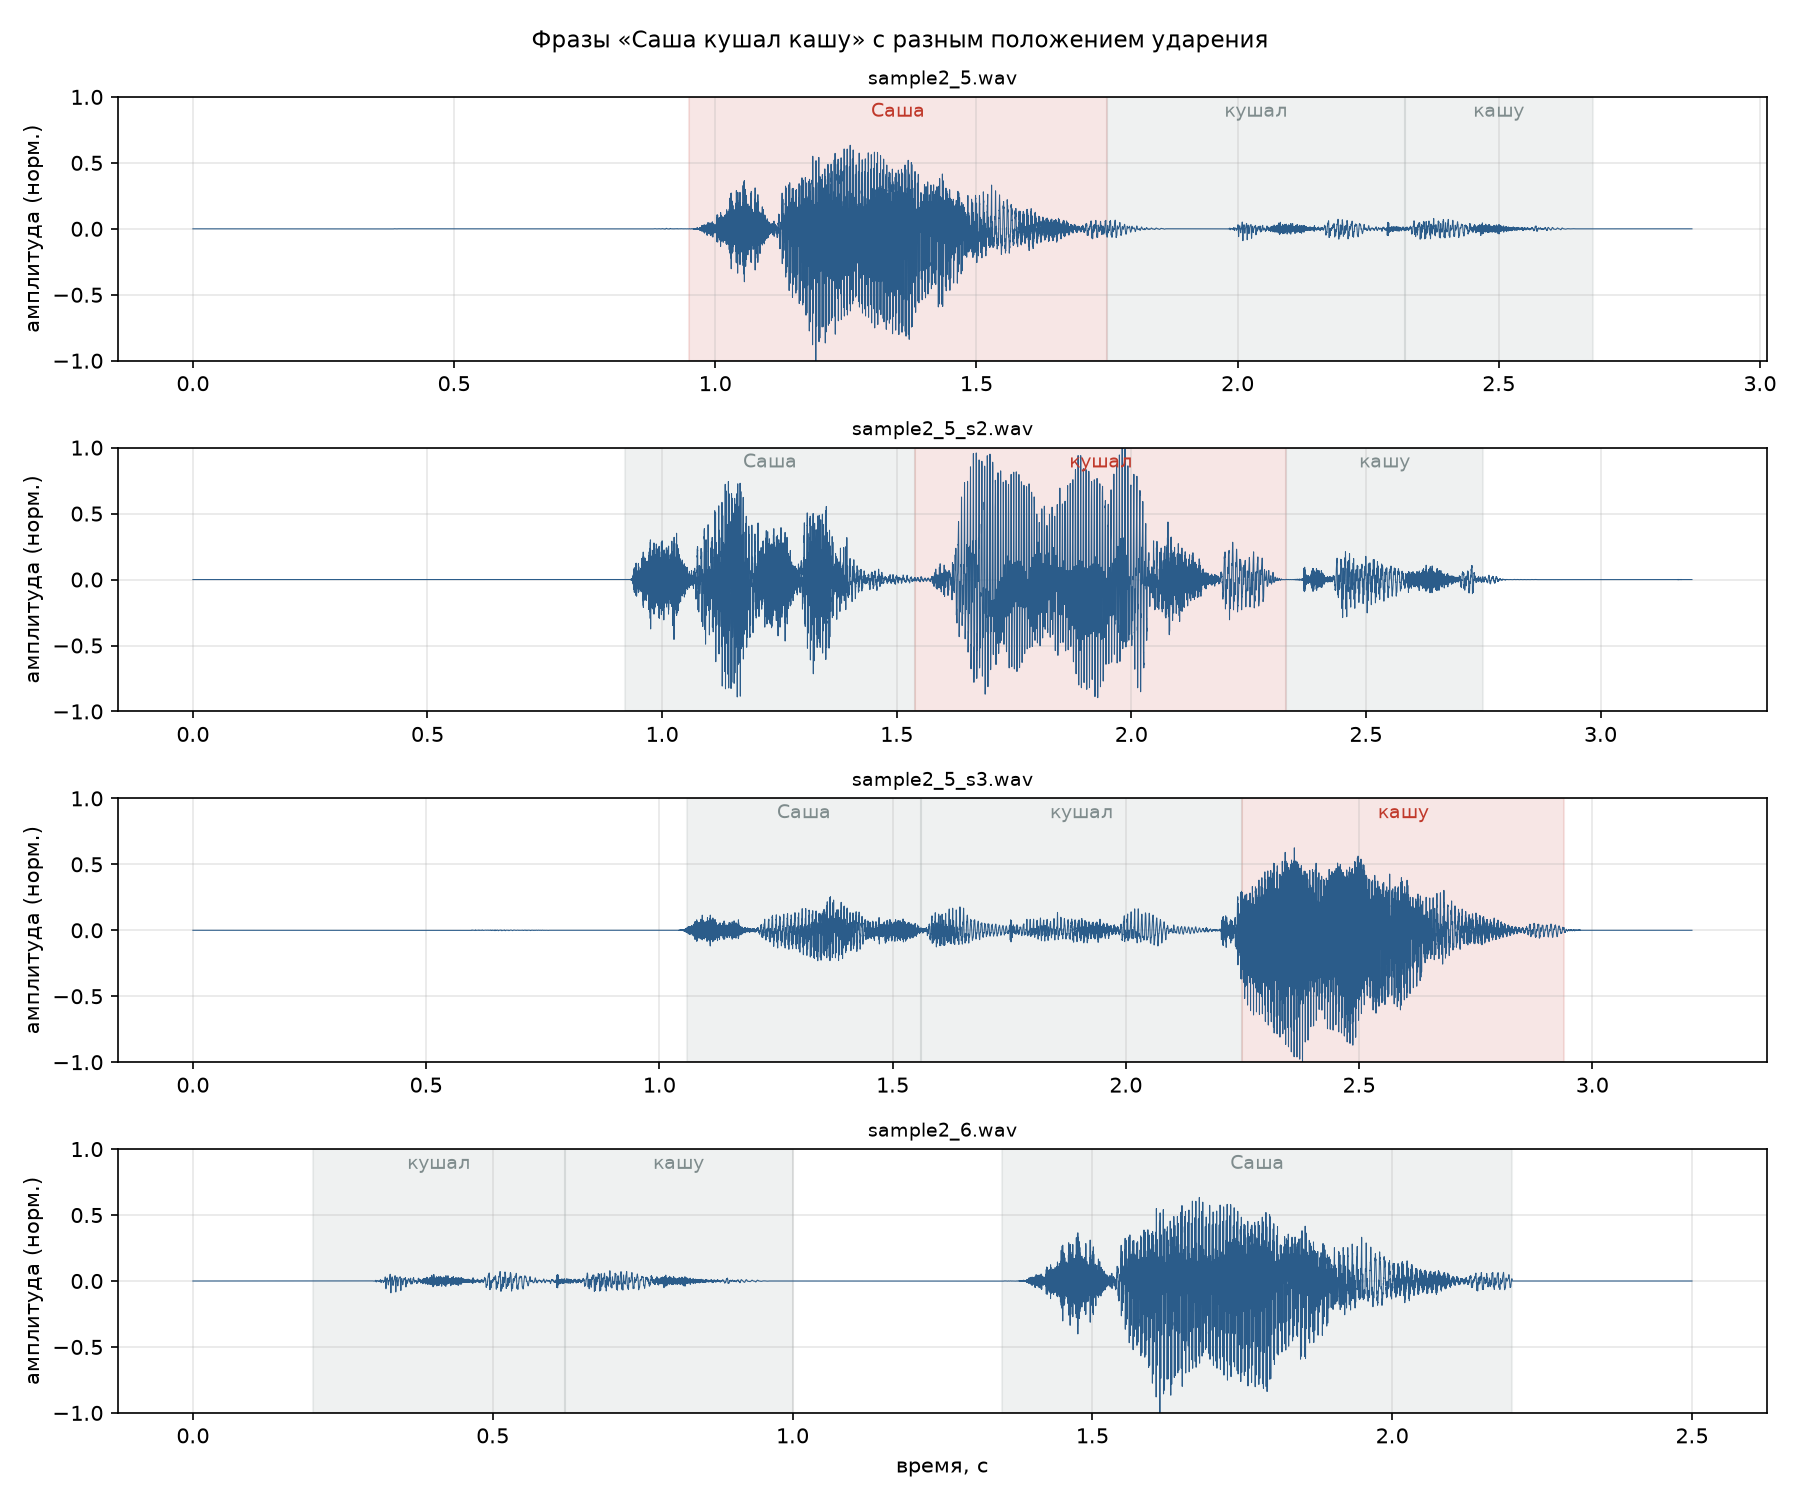
\includegraphics[width=\textwidth]{lab2_stress_waves.png}
	\caption{Осциллограммы фраз <<Саша кушал кашу>> с ударением на первое,
		второе и третье слово и с переносом слова <<Саша>> в конец}
	\label{fig:stress-waves}
\end{figure}

\begin{figure}[H]
	\centering
	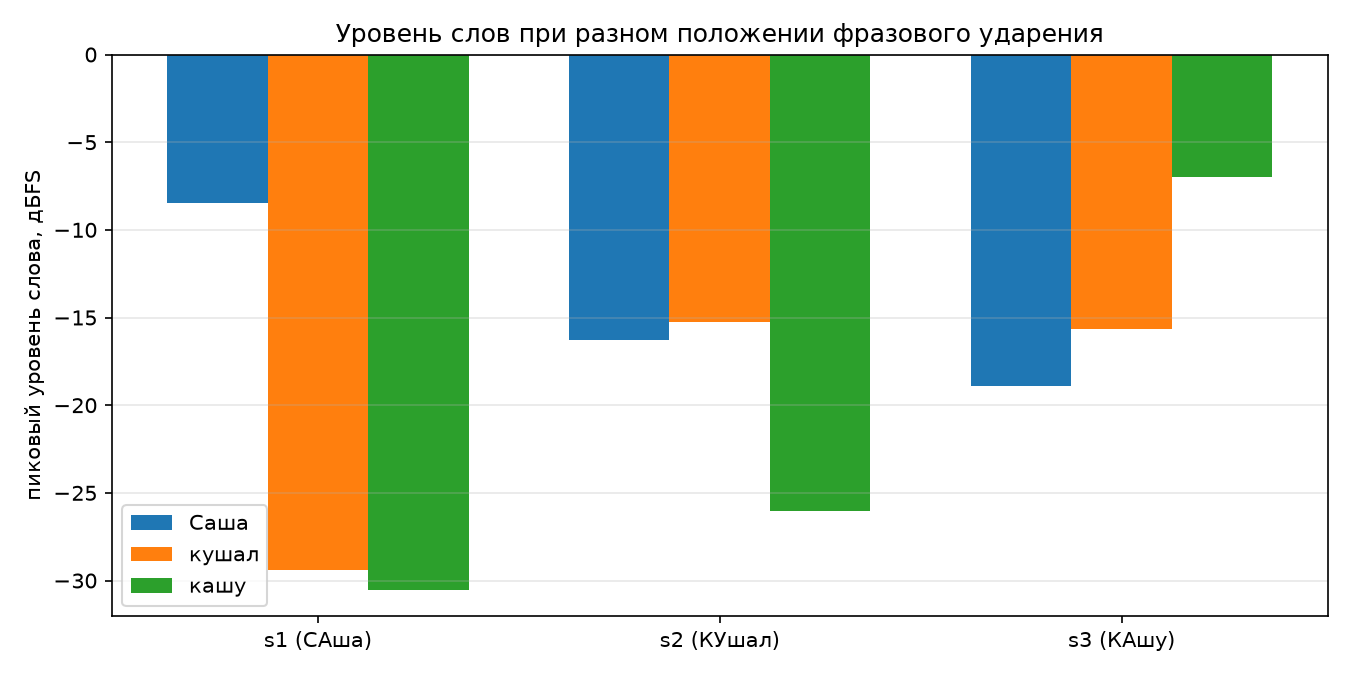
\includegraphics[width=\textwidth]{lab2_accent_levels.png}
	\caption{Пиковые уровни слов при разном положении фразового ударения}
	\label{fig:accent-levels}
\end{figure}

Таким образом, ударение в речевом сигнале проявляется комплексно:
ударный слог (слово) имеет повышенный уровень (на 10--20~дБ), увеличенную
длительность и, как правило, повышенную частоту основного тона
(145--167~Гц против 112--133~Гц у безударных слов). При перестановке слов
интонационный рисунок сохраняется --- фраза по-прежнему состоит из трёх
акцентных групп, --- а перенос ударного слова в конец меняет вид
акцентной группы и восприятие фразы (утверждение превращается в вопрос).

\subsection{Задание 2.2.2. Явление интонации}

Фраза <<Саша кушал кашу>> записана с четырьмя видами интонации:
простая завершённость (.), незавершённость (,) --- фраза продолжена
словами <<сегодня на обед>>, вопрос (?) и восклицание (!). Дополнительно
записаны эмоционально окрашенные варианты: с чувством радости и с
огорчением.

Мелодические контуры $F_0$, рассчитанные по записям, приведены на
рис.~\ref{fig:intonation}. Количественные характеристики --- медиана и
максимум $F_0$, положение мелодического максимума (в долях длительности
речи) и изменение тона в конце фразы --- сведены в
таблицу~\ref{tab:intonation}.

\begin{table}[H]
	\centering
	\caption{Характеристики мелодических контуров для разных
		интонационных типов}
	\label{tab:intonation}
	\small
	\begin{tabular}{|l|l|l|l|l|l|}
		\hline
		Интонация & Длит., с & Медиана $F_0$, Гц & Макс. $F_0$, Гц &
		Поз. макс. & $\Delta F_0$, пт \\
		\hline
		завершённость (.) & 2,04 & 130 & 170 & 0,24 & $-4{,}7$ \\
		\hline
		незавершённость (,) & 3,24 & 127 & 165 & 0,05 & $-2{,}1$ \\
		\hline
		вопрос (?) & 1,60 & 120 & 232 & 0,94 & $+6{,}7$ \\
		\hline
		восклицание (!) & 1,50 & 142 & 193 & 0,09 & $-1{,}1$ \\
		\hline
	\end{tabular}
\end{table}

\begin{figure}[H]
	\centering
	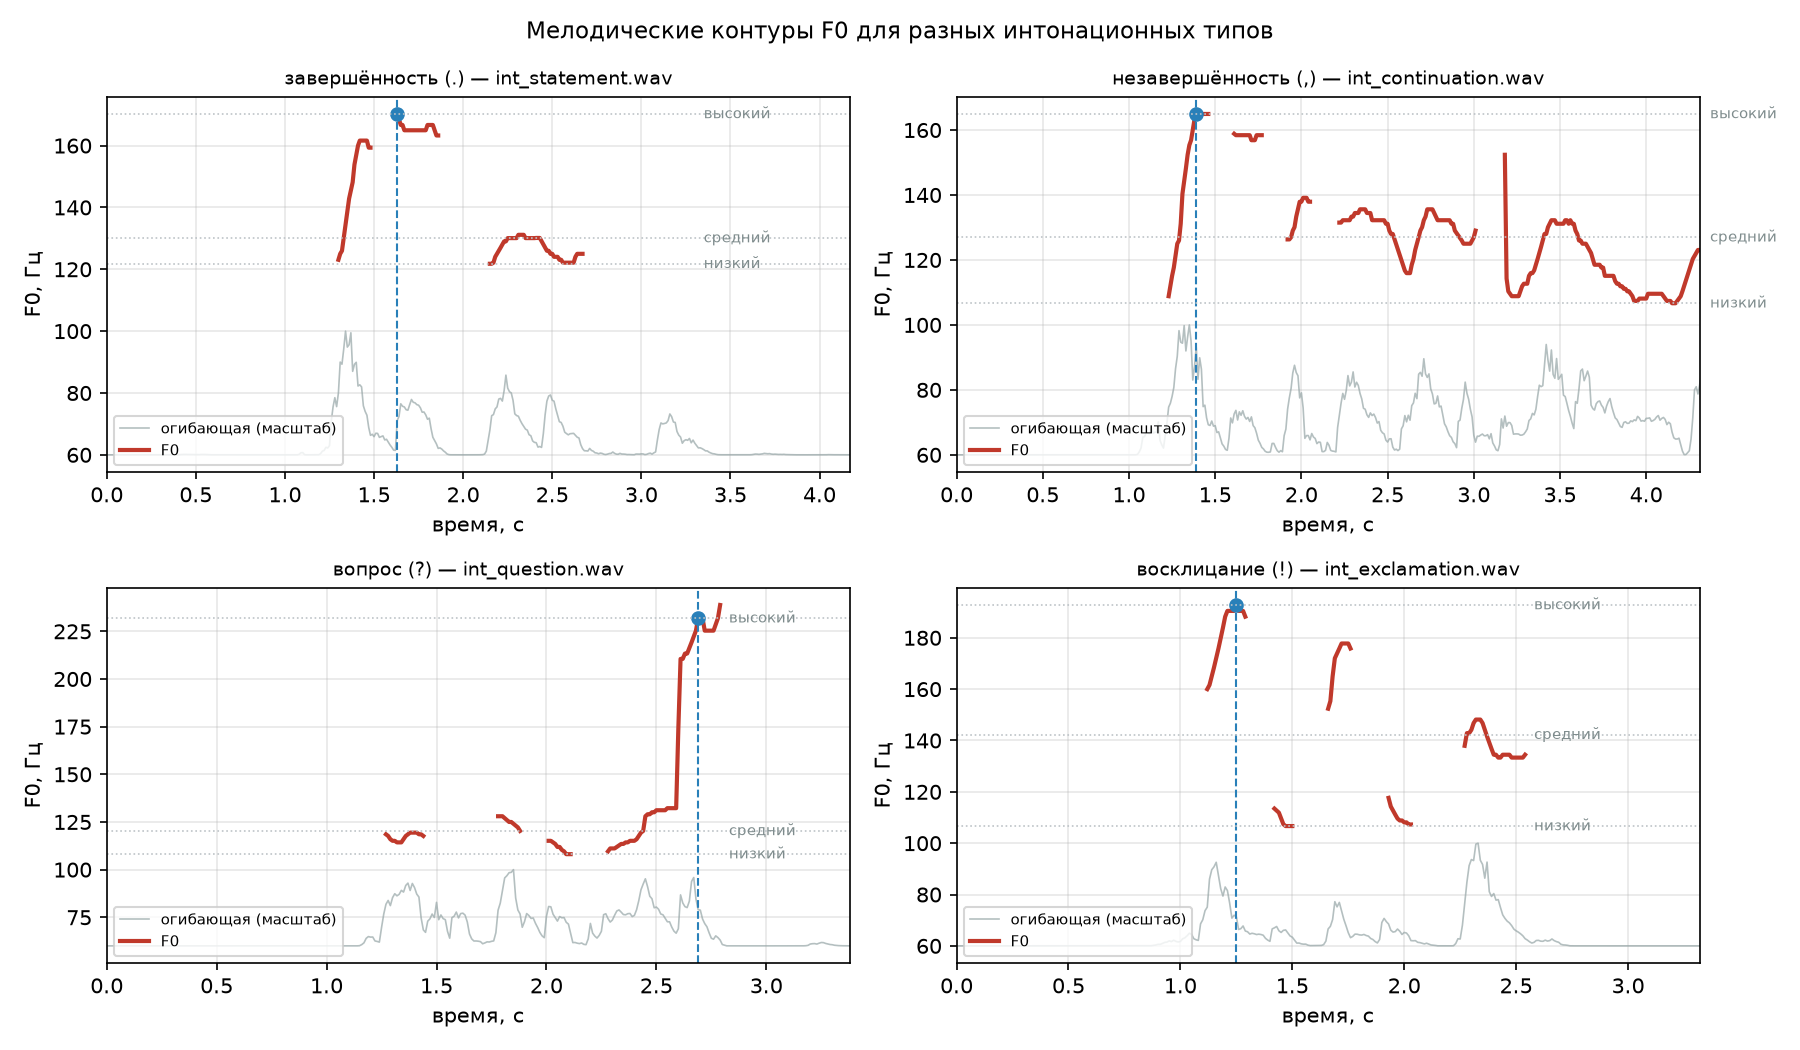
\includegraphics[width=\textwidth]{lab2_intonation_contours.png}
	\caption{Мелодические контуры $F_0$ для интонаций завершённости,
		незавершённости, вопроса и восклицания}
	\label{fig:intonation}
\end{figure}

Полученные результаты согласуются с теоретической схемой интонационных
типов:
\begin{itemize}
	\item при интонации \emph{завершённости} мелодический максимум
	расположен в начале фразы (0,24), а к концу тон понижается на
	4,7~полутона --- типичный нисходящий терминальный контур;
	\item при \emph{вопросе} максимум смещён к концу фразы (0,94), а тон в
	конце повышается на 6,7~полутона: наблюдается отчётливый восходящий
	терминальный контур, что и делает фразу вопросом;
	\item при \emph{восклицании} фраза начинается с высокого тона
	(максимум 193~Гц в начале) и затем тон понижается --- высокий
	энергичный зачин с падением;
	\item при \emph{незавершённости} контур занимает промежуточное
	положение: тон не получает завершающего падения, а фраза продолжается
	следующей синтагмой.
\end{itemize}

\begin{figure}[H]
	\centering
	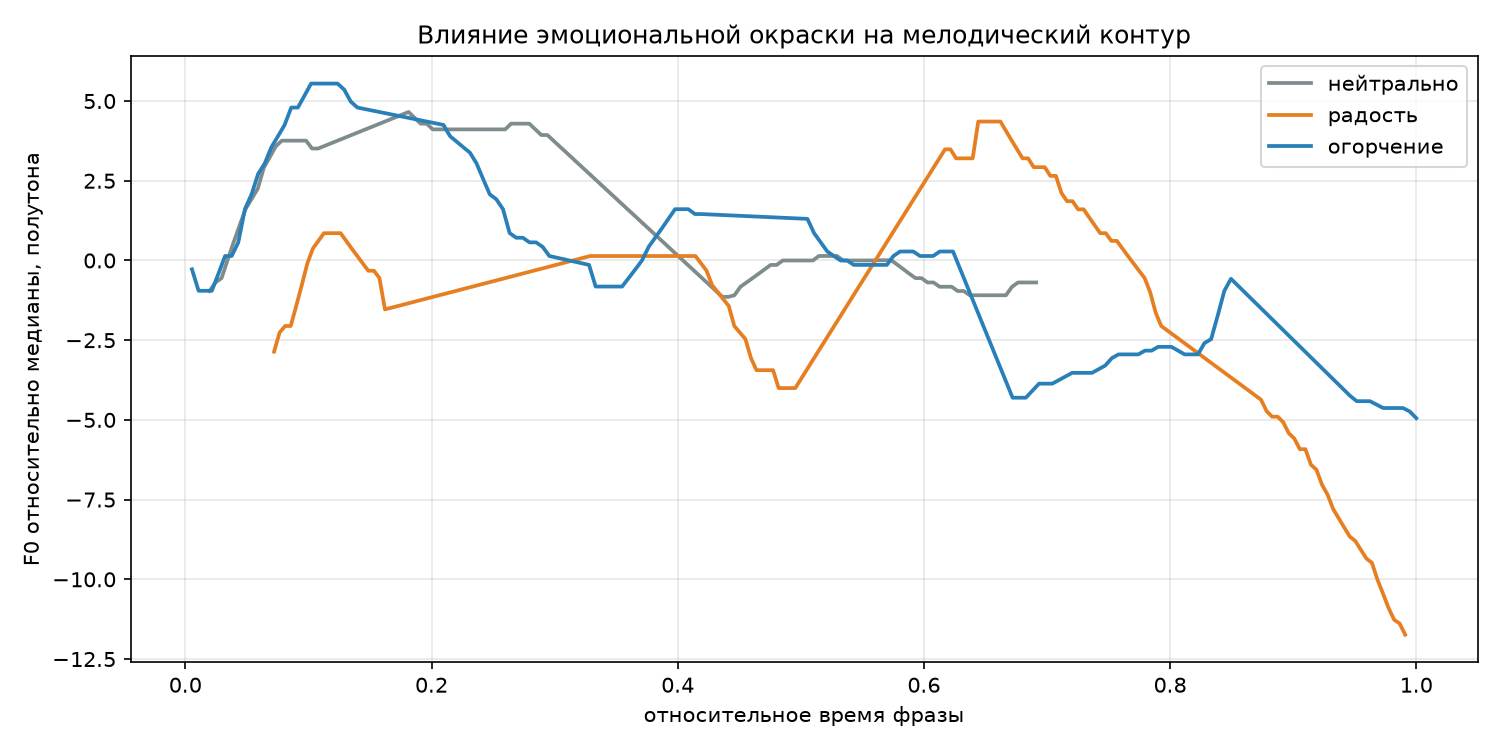
\includegraphics[width=\textwidth]{lab2_emotion_contours.png}
	\caption{Влияние эмоциональной окраски на мелодический контур фразы}
	\label{fig:emotion}
\end{figure}

Сравнение эмоционально окрашенных вариантов (рис.~\ref{fig:emotion})
показывает, что эмоции изменяют не столько средний уровень тона, сколько
\emph{диапазон} его изменения: при радости наблюдаются более резкие
подъёмы и глубокие спады $F_0$, при огорчении контур более плавный.
Таким образом, просодические характеристики (ударение и интонация)
непосредственно влияют на речевой сигнал и передают смысловую и
эмоциональную информацию.

\subsection{Задание 2.2.1, п.~14 и 2.2.2, п.~4: проверка на собственном
	материале}

Чтобы проверить сделанные выводы на материале, который не входил в
постановку задания, дополнительно записаны длинная фраза <<Сегодня утром
студенты сдали экзамен по теории вероятностей>> и пара коротких фраз
<<Ты дома?>> и <<Ты дома.>>, произнесённых с разной интонацией. Запись
выполнена в той же сессии и с теми же параметрами (16~кГц, моно,
16~бит), фразы разделены паузами и нарезаны автоматически по тишине.

\subsubsection{Акцентные группы в длинной фразе}

Границы акцентных групп определялись автоматически по глубоким минимумам
кратковременной энергии, соответствующим паузам между синтагмами:
минимумы с перепадом более 40~дБ приходятся на 1,12 и 2,68~с, что делит
фразу на три группы. Для каждой группы измерены длительность, пиковый и
средний уровень, медиана и максимум $F_0$, а также положение главного
ударного слога (максимум кратковременной энергии). Результаты сведены в
таблицу~\ref{tab:extra-accents}, осциллограмма и контур $F_0$ с
границами групп --- на рис.~\ref{fig:extra-accents}.

\begin{table}[H]
	\centering
	\small
	\caption{Акцентные группы в длинной фразе}
	\label{tab:extra-accents}
	\begin{tabular}{|l|l|l|l|l|}
		\hline
		Группа & Интервал, с & Длит., с & Пик / RMS, дБFS &
		$F_0$ медиана / макс., Гц \\
		\hline
		АГ1 & 0,00--1,12 & 1,12 & $-11{,}5$ / $-25{,}4$ & 113 / 136 \\
		\hline
		АГ2 & 1,12--2,68 & 1,56 & $-11{,}8$ / $-27{,}6$ & 144 / 205 \\
		\hline
		АГ3 & 2,68--3,78 & 1,10 & $-13{,}6$ / $-27{,}2$ & 120 / 143 \\
		\hline
	\end{tabular}
\end{table}

\begin{figure}[H]
	\centering
	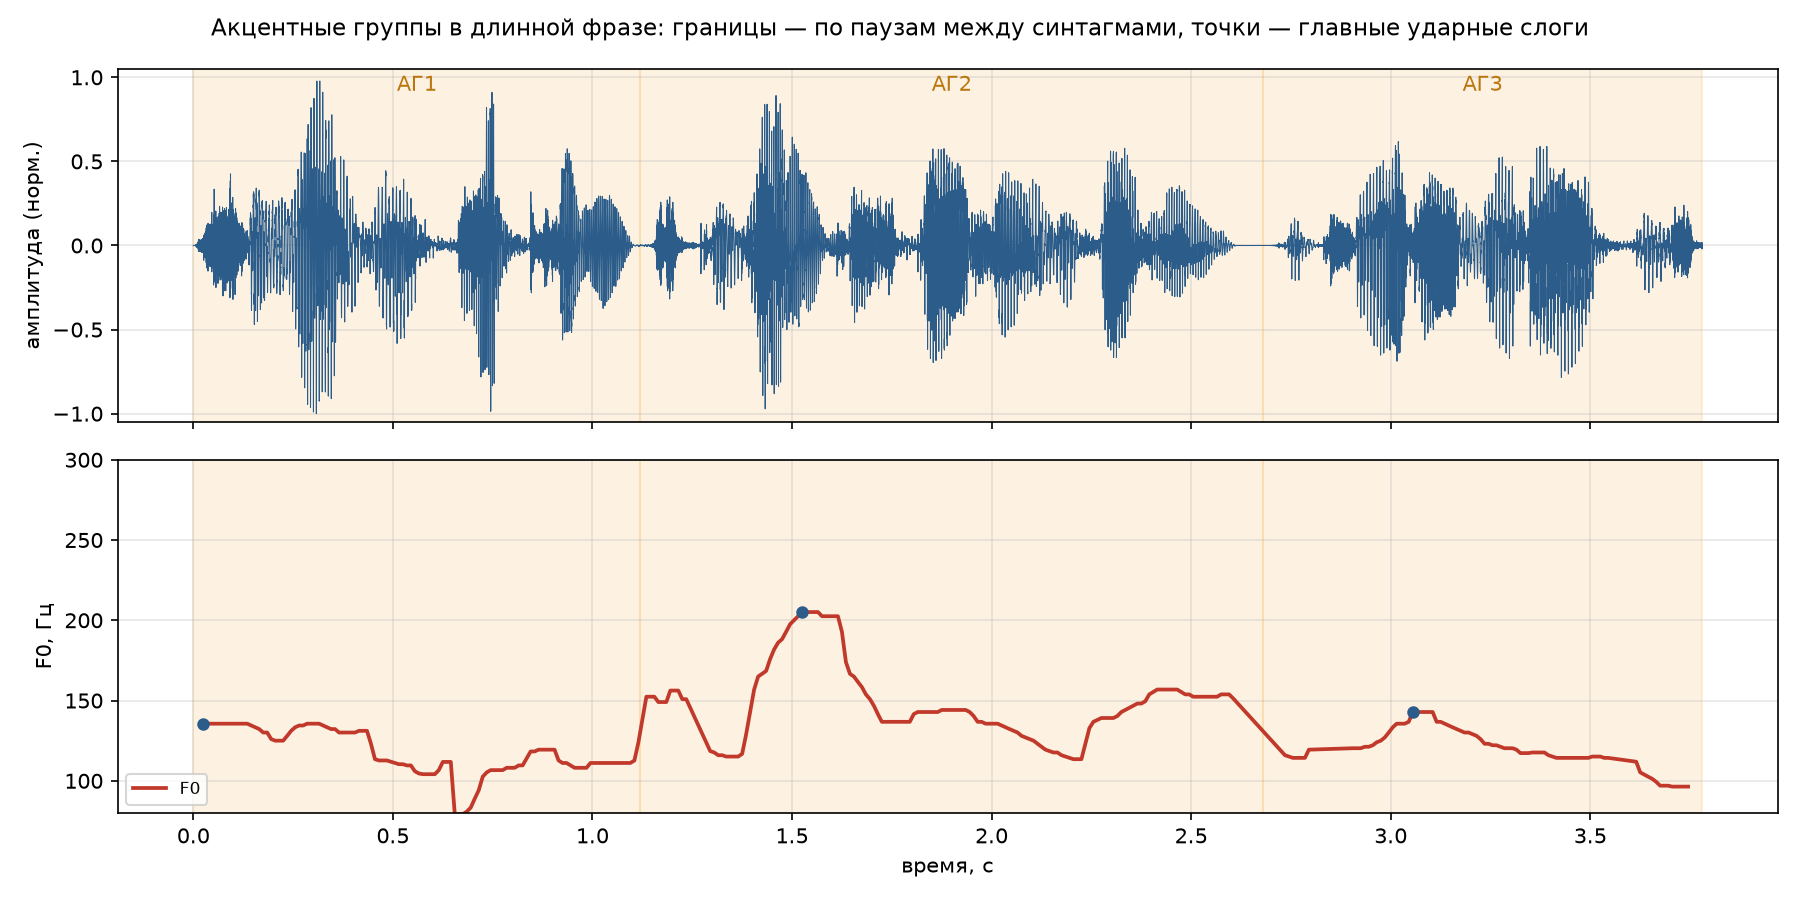
\includegraphics[width=\textwidth]{lab2_extra_accents.png}
	\caption{Акцентные группы в длинной фразе: осциллограмма, контур $F_0$
		и главные ударные слоги (точки)}
	\label{fig:extra-accents}
\end{figure}

Группы неравноправны: вторая группа самая длинная (1,56~с) и наиболее
выделенная по тону --- медиана 144~Гц против 113 и 120~Гц, максимум
205~Гц, тогда как в первой и третьей группах максимум не превышает
143~Гц. Именно она несёт логическое ударение высказывания. Третья
группа замыкает фразу и имеет наименьший пиковый уровень
($-13{,}6$~дБFS) --- типичное ослабление к концу высказывания. При этом
каждая группа содержит собственный ударный слог, то есть длинная фраза
действительно членится на несколько акцентных групп, каждая из которых
может быть записана как $(+)$.

\subsubsection{Вопрос и утверждение}

Одна и та же фраза <<Ты дома>> произнесена дважды: с вопросительной
интонацией и с интонацией утверждения. Параметры контуров приведены в
таблицу~\ref{tab:extra-qs}, сами контуры --- на рис.~\ref{fig:extra-qs}.

\begin{table}[H]
	\centering
	\small
	\caption{Мелодические контуры одной фразы при разной интонации}
	\label{tab:extra-qs}
	\begin{tabular}{|l|l|l|l|l|l|l|}
		\hline
		Фраза & Нач., Гц & Макс., Гц & Поз. макс. &
		Кон., Гц & Рост, пт & Спад, пт \\
		\hline
		вопрос & 129 & 271 & 0,59 & 116 & $+12{,}9$ & $-14{,}7$ \\
		\hline
		утверждение & 126 & 154 & 0,37 & 106 & $+3{,}5$ & $-6{,}5$ \\
		\hline
	\end{tabular}
\end{table}

\begin{figure}[H]
	\centering
	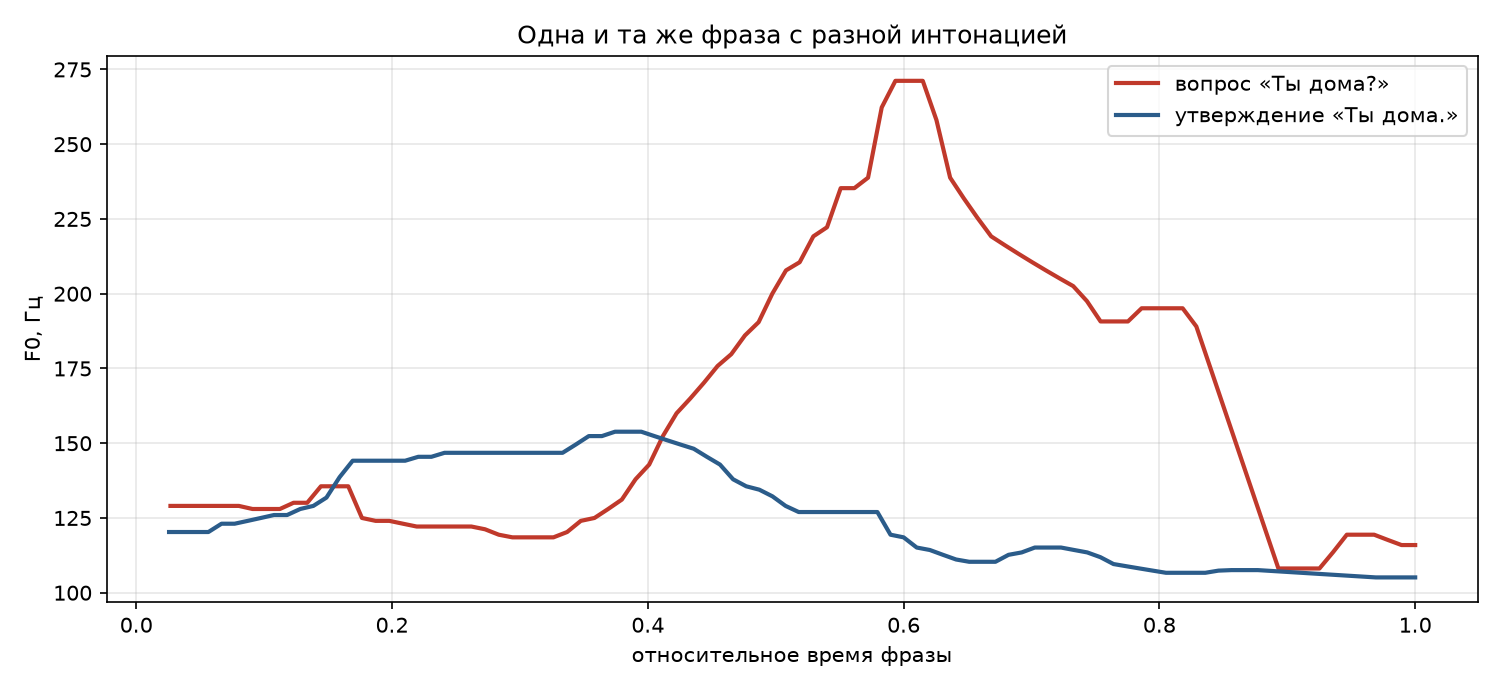
\includegraphics[width=\textwidth]{lab2_extra_qs.png}
	\caption{Контуры $F_0$ фразы <<Ты дома>> при вопросительной интонации
		и интонации утверждения}
	\label{fig:extra-qs}
\end{figure}

Контуры расходятся прежде всего в области ударного гласного: в вопросе
тон поднимается с 129 до 271~Гц (на 12,9~полутона) и затем падает на
14,7~полутона, тогда как в утверждении максимум составляет лишь
154~Гц (подъём 3,5~полутона) и контур плавно понижается к 106~Гц.
Диапазон изменения тона в вопросе вдвое больше (11,6 против
5,6~полутона), а мелодический максимум смещён вправо (0,59 против
0,37 длительности фразы). Последнее согласуется с правилом, выведенным
по фразе <<Саша кушал кашу>>: при вопросе максимум $F_0$ смещается к
концу высказывания.

Отметим, что в этой записи вопрос реализован подъёмом на ударном
гласном с последующим падением (тип ИК-3), а не терминальным подъёмом,
как в ранее проанализированной фразе <<Саша кушал кашу>>, где максимум
приходился на 0,94 длительности. Это показывает, что вопросительная
интонация имеет несколько мелодических вариантов; однако во всех
случаях вопросительная фраза отличается от утвердительной смещением
мелодического максимума вправо и большим диапазоном изменения $F_0$.
